\documentclass{beamer}
\usetheme{Madrid}


\usepackage{comment}
\usepackage{amsmath, amssymb}  
\usepackage{amsthm}  
\usepackage{mathtools}  
\usepackage{complexity}

\newcommand{\cetal}{\textit{et al.\@}}  % shortcut for etal to be used when no space is desired
\newcommand{\etal}{\textit{et al.\@\ }}  % shortcut for etal to be used in regular text
\newcommand{\nrank}{\operatorname{rank}_+}
\newcommand{\rank}{\operatorname{rank}}
\newcommand{\diag}{\operatorname{diag}}
\newcommand{\bits}{\{0,1\}}
\newcommand{\abs}[1]{\left|#1\right|}
\newcommand{\conv}{\operatorname{conv}}
\newcommand{\suppmat}{\operatorname{suppmat}}
\newcommand{\supp}{\operatorname{supp}}
\newcommand{\ol}[1]{\overline{#1}}
\newcommand{\ul}[1]{\underline{#1}}
\newcommand{\oul}[1]{\overline{\underline{#1}}}
\newcommand{\xc}{\operatorname{xc}}
\newcommand{\TSP}{\operatorname{TSP}}
\newcommand{\STAB}{\operatorname{STAB}}
\newcommand{\CUT}{\operatorname{CUT}}
\newcommand{\COR}{\operatorname{COR}}
\renewcommand{\R}{\mathbb{R}}

\newenvironment{proofsketch}{%
  \renewcommand{\proofname}{Proof Sketch}\proof}{\endproof}


\author[Livanos, Torres]{Vasilis Livanos and Manuel Torres}
\title[Exp. Lower Bounds for Polytopes]{Exponential Lower Bounds for Polytopes in Combinatorial Optimization}
\institute[UIUC]{University of Illinois at Urbana-Champaign}
\date{May 2, 2018}

\begin{document}

\begin{frame}
\titlepage
\end{frame}


\begin{frame}
\frametitle{Main Question}

\pause
\begin{itemize}
\item Let's prove $\P = \NP$!
\pause
\item Idea: Can we write a polynomial-size LP (Linear Program) for an \NP-Complete problem (e.g. $\lang{TSP}$)?
\pause
\item Another idea: Encode a problem as a polytope that is the convex hull of the vertices corresponding to the solutions of the problem.
\end{itemize}
\end{frame}


\begin{frame}
\frametitle{Necessary Background}

\pause
\begin{definition}[Extended Formulation]
Let $P = \{x : Ax \leq b\}$ and $Q = \{(x,y) : Bx + Cy \leq d\}$. Then $Q$ is an \emph{extended formulation (EF)} of $P$ if and only if
\[
P = \{x : \exists y , (x,y) \in Q\}
\]
The size of an extended formulation is the number of facets (faces of maximal dimension) of $Q$.
\end{definition}

\pause
\begin{definition}[Extension Complexity]
The \emph{extension complexity} of $P$, denoted $\xc(P)$, is the minimum size EF of $P$.
\end{definition}

\end{frame}


\begin{frame}
\frametitle{Extended Formulations Can Help}

\pause
\begin{itemize}
\item There are polytopes that have exponential size (i.e. number of facets), but have an EF with polynomial size.
\pause
\begin{enumerate}
\item The permutahedron polytope, which is the convex hull of the permutation group on $\{1, 2, \ldots, n\}$.
\pause
\item The spanning tree polytope.
\pause
\item The matching polytope for planar graphs.
\end{enumerate}
\pause
\item Thus, even though these polytopes have exponential size, we can write a polynomial-size LP for them, through their EF.
\end{itemize}
\end{frame}


\begin{frame}
\frametitle{Prior Work}

\pause
\begin{theorem}[Yannakakis, '91]
Every symmetric LP for TSP has extension complexity $2^{\Omega(n)}$. Thus, it also has an exponential number of inequalities.
\end{theorem}

\pause
\begin{corollary}
No symmetric LP can be used to solve TSP in polynomial time.
\end{corollary}

\pause
\begin{itemize}
\item Can we use an asymmetric LP to solve TSP in polynomial time?
\end{itemize}

\end{frame}


\begin{frame}
\frametitle{More Technical Background}

\pause
\begin{definition}[Nonnegative Rank]
Let $M \in \R_+^{m \times n}$. The \emph{nonnegative rank} of $M$ is defined as $\nrank(M) = \min\{r : M = TU, T \in \R_+^{m \times r}, U \in \R_+^{r \times n}\}$.
\end{definition}

\pause
\begin{definition}[Slack Matrix]
Let $A \in \R^{m \times d}$, $b \in \R^m$, and $V = \{v_1, \ldots, v_n\} \subseteq \R^d$. Let $P = \{x \in \R^d : Ax \le b\} = \conv(V)$. Then $S \in \R_+^{m\times n}$, where each entry is defined as $S_{ij} = b_i - A_i v_j$ with $i \in [m]$, $j \in [n]$, is the \emph{slack matrix} of $P$ with respect to $Ax \le b$ and $V$.
\end{definition}

\end{frame}


\begin{frame}
\frametitle{Yannakakis's Factorization Theorem}

\pause
\begin{theorem}[Factorization Theorem, Yannakakis '91]
Let $P = \left\{ x \in \R^d \mid Ax \leq b \right\} = \conv(V)$ be a polytope, and $S$ be its slack matrix with respect to $Ax \leq b$ and $V$. Then
\[
\xc(P) = \nrank(S)
\]
\end{theorem}

\pause
\begin{itemize}
\item If we want to lower bound $\xc(P)$, it suffices to lower bound $\nrank(S)$.
\end{itemize}

\end{frame}


\begin{frame}
\frametitle{Lower Bound on Nonnegative Rank}

\pause
\begin{definition}[Support Matrix]
The {\em support matrix} of a matrix $M$ with nonnegative entries is
\[
\suppmat(M)_{ij} = \begin{cases}
0 & M_{ij} = 0 \\
1 & M_{ij} \neq 0
\end{cases}
\]
\end{definition}

\pause
\begin{theorem}[Yannakakis, '91]
Let $M$ be a matrix with nonnegative entries, and $\suppmat(M)$ its support matrix.
Then, $\nrank(M)$ is lower bounded by the rectangle covering bound for $\suppmat(M)$.
\end{theorem}

\pause
\begin{itemize}
\item This provides a connection between $\xc(P)$ and communication complexity.
\end{itemize}

\end{frame}


\begin{frame}
\frametitle{Reminder: Rectangle Covers}

\pause
\begin{definition}[Rectangle Cover]
Let $M \in \bits^{2^n \times 2^n}$ with indices corresponding to bit strings. A \emph{rectangle} is a subset of $\bits^n \times \bits^n$. We say that $R \subseteq \bits^n \times \bits^n$ is a \emph{$b$-monochromatic rectangle} for $f$ if $M_{xy} = b$ for all $(x,y) \in R$. We say that a set $\mathcal{R}$ of $b$-monochromatic rectangles is a \emph{$b$-rectangle cover} if $\{(x,y) \in \bits^n \times \bits^n : M_{xy} = b\} \subseteq \bigcup_{R \in \mathcal{R}} R$.
\end{definition}

\end{frame}


\begin{frame}
\frametitle{A Matrix of Exponential Nonnegative Rank}

\pause
\begin{definition}
Let $M$ be a $2^n \times 2^n$ matrix, where each row (resp. column) is indexed by a $n$-bit string $a$ (resp. $b$), with
\[
M_{ab} \coloneqq {\left(1 - a^Tb\right)}^2
\]
\end{definition}

\pause
\begin{theorem}[De Wolf, '03]
Every $1$-monochromatic rectangle cover of $\suppmat(M)$ has size $2^{\Omega(n)}$.
\end{theorem}

\end{frame}


% !TEX root = main.tex 

\begin{frame}
\frametitle{$\CUT(n)$ and $\COR(n)$ Polytopes}
\onslide<1->{
\begin{definition}[cut polytope]
Let $K_n = (V,E)$ be the complete graph on $n$ vertices. Let $\delta(S)$ denote the cut of $S \subseteq V$. Then let $\chi^{\delta(S)} \in \R^{\abs{E}}$ such that
\[
\chi^{\delta(S)}_e =
\begin{cases}
1 & e \in \delta(S) \\
0 & e \notin \delta(S)
\end{cases}.
\]
Then $\CUT(n) \coloneqq \conv\left( \left\{ \chi^{\delta(S)} \in \R^{\abs{E}} \mid S \subseteq V \right\} \right)$
\end{definition}
}
\onslide<2->{
\begin{definition}[correlation polytope]
We have $\COR(n) \coloneqq \conv\left( \left\{ bb^T \in \R^{n \times n} \mid b \in {\{0, 1\}}^n \right\} \right)$
\end{definition}
}
\end{frame}

\begin{frame}
\frametitle{Connection Between $\CUT(n)$ and $\COR(n)$}
\onslide<1->{
\begin{definition}[linearly isomorphic polytopes]\label{def:lin-iso}
Two polytopes $P \subseteq \R^n$ and $Q \subseteq \R^m$ are called \textit{linearly isomorphic} if there exists a linear invertible function $f : \R^n \to \R^m$ such that $f(P) = Q$.
\end{definition}
}
\onslide<2->{
\begin{lemma}[De Simone, '90]
For all $n$, $\COR(n)$ is linearly isomorphic to $\CUT(n+1)$.
\end{lemma}
}

\onslide<3->{
\begin{corollary}
$\xc(\COR(n)) = \xc(\CUT(n+1))$.
\end{corollary}
}
\end{frame}

\begin{frame}
\frametitle{$\CUT(n)$ has Exponential Extension Complexity}

\onslide<1->{
\begin{theorem}
The extension complexity of $\CUT(n)$ is $2^{\Omega(n)}$.
\end{theorem}
}

\onslide<2->{
\onslide
\begin{proofsketch}
\begin{enumerate}
\item<2-> $\xc(\COR(n)) = \xc(\CUT(n+1))$ 
\item<3-> $\xc(\COR(n)) = \nrank(S)$ where $S$ is the slack matrix of $\COR(n)$
\item<4-> $\nrank(S) \ge \nrank(M)$ 
\item<5-> $\nrank(M) = 2^{\Omega(n)}$.
\end{enumerate}
\vspace{-4mm}
\end{proofsketch}
}

\end{frame}

\begin{frame}
\frametitle{Reductions}
\begin{lemma}
Let $P$ and $F$ be polytopes. If $F$ is a face of $P$, then $\xc(P) \ge \xc(F)$.
\end{lemma}
\end{frame}

\begin{frame}
\frametitle{$\STAB(G)$ Reduces to $\COR(n)$}
\begin{definition}[Stable Set Polytope]
The \emph{stable set polytope} $\STAB(G)$ is defined as the convex hull of the characteristic vectors of all stable sets in $G = (V, E)$. That is,
\[
\STAB(G) \coloneqq \conv\left(\left\{\chi^S \in \R^V \mid S \text{ is a stable set of $G$}\right\}\right).
\]
\end{definition}
\end{frame}

\begin{frame}
\frametitle{Reduction from $\STAB(G)$ to $\COR(n)$}
\begin{itemize}
\item<1-> We will construct a graph $H_n$
\item<2-> Let $K_n$ be the complete graph on the vertices $[n]$
\item<3-> For an edge $\{i,j\}$ in $K_n$ where $i < j$, label the edge $ij$
\item<4-> The vertex set of $H_n$ is
\[
V = \{ii, \ol{ii} : i \in [n]\} \cup \{ij, \ol{ij}, \ul{ij}, \oul{ij}, : i,j \in [n], i < j\}.
\]
\end{itemize}
\end{frame}

\begin{frame}
\frametitle{Reduction from $\STAB(G)$ to $\COR(n)$ (cont.)}
\begin{figure}
\centering
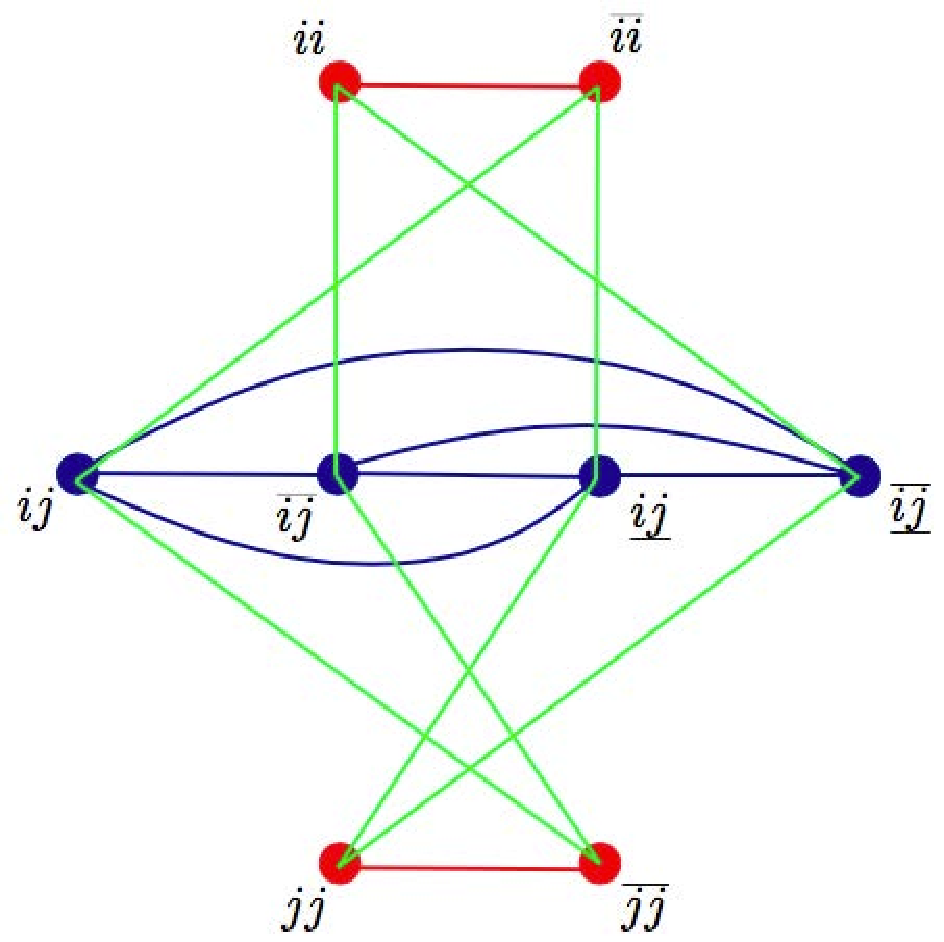
\includegraphics[scale=0.35]{stable.pdf}
\caption{the set of edges and vertices added to $H_n$ for some $i,j \in [n]$ with $i < j$.}
\end{figure}
\end{frame}

\begin{frame}
\frametitle{Reduction from $\STAB(G)$ to $\COR(n)$ (cont.)}

\begin{lemma}
$\STAB(H_n)$ contains a face that is an extension of $\COR(n)$.
\end{lemma}
\end{frame}

\begin{frame}
\frametitle{Extension Complexity of $\STAB(G)$ is $2^{\Omega(\sqrt{n})}$}

\onslide<1->{
\begin{theorem}
For all $n$, there exists a graph $G_n$ with $n$ vertices such that $\xc(\STAB(G_n)) = 2^{\Omega(\sqrt{n})}$.
\end{theorem}
}

\onslide<2->{
\onslide
\begin{proofsketch}
\begin{enumerate}
\item<2-> Let $G_n$ be $H_\ell$ with $n - O(\ell^2)$ isolated vertices \onslide<3->{$\Rightarrow \ell = \Omega(\sqrt{n})$}
\item<4-> $\xc(\STAB(G_n)) \ge \xc(\STAB(H_\ell))$ 
\item<5-> $\xc(\STAB(H_\ell)) \ge \xc(\COR(\ell))$
\item<6-> $ \xc(\COR(\ell)) = 2^{\Omega(\ell)}$
\item<7-> $2^{\Omega(\ell)} = 2^{\Omega(\sqrt{n})}$.
\end{enumerate}
\vspace{-4mm}
\end{proofsketch}
}
\end{frame}







\begin{frame}
\frametitle{$\TSP(n)$ Polytope}

\pause
\begin{definition}[$\TSP$ Polytope]
Let $K_n = (V_n, E_n)$ be the complete graph with $n$ vertices. The \emph{Traveling Salesman Problem polytope} $\TSP(n)$ is defined as the convex hull of the characteristic vectors of all $F \subseteq E_n$ such that $F$ is a Hamiltonian cycle of $K_n$. In other words,
\[
\TSP(n) \coloneqq \conv\left(\left\{\chi^F \in \R^{E_n} \mid F \subseteq E_n \text{ is a Hamiltonian cycle of $K_n$}\right\}\right).
\]
\end{definition}

\pause
\begin{itemize}
\item Intuitively, the $\TSP(n)$ polytope is the polytope that has every Hamiltonian cycle of $K_n$ as a vertex.
\end{itemize}

\end{frame}

\begin{frame}
\frametitle{$\TSP(n)$ Polytope}

\pause
\begin{lemma}
For every $n$, there exists a positive integer $q = O(n^2)$ such that $\COR(n)$ is contained in a face of $\TSP(q)$.
\end{lemma}

\pause
\begin{theorem}
The extension complexity of $\TSP(n)$ is $\xc\left(\TSP(n)\right) = 2^{\Omega\left(\sqrt{n}\right)}$.
\end{theorem}

\end{frame}

% !TEX root = main.tex 

\begin{frame}
\frametitle{Subsequent Work}

\begin{itemize}
\item<1-> Rhothvo{\ss} showed that the matching polytope has extension complexity $2^{\Omega(n)}$
\item<2-> In this work, he also showed that the extension complexity of $\TSP(n)$ is $2^{\Omega(n)}$.
\item<3-> Braverman and Moitra showed that any linear program that attains an $O(n^{1-\epsilon})$ approximation for Max-Clique has size $2^{\Omega(n^\epsilon)}$.
\end{itemize}
\end{frame}







\begin{frame}
\begin{center}
\LARGE{QUESTIONS ?}
\end{center}
\begin{figure}
        \centering
        \begin{minipage}{.5\textwidth}
            \centering
            
\includegraphics[width=.8\linewidth]{questions.png}
        \end{minipage}%
        
\end{figure}
\end{frame}

\end{document}
